\documentclass[tikz, mode=buildnew]{standalone}
\usetikzlibrary{arrows.meta, graphs, shapes.geometric}

\begin{document}
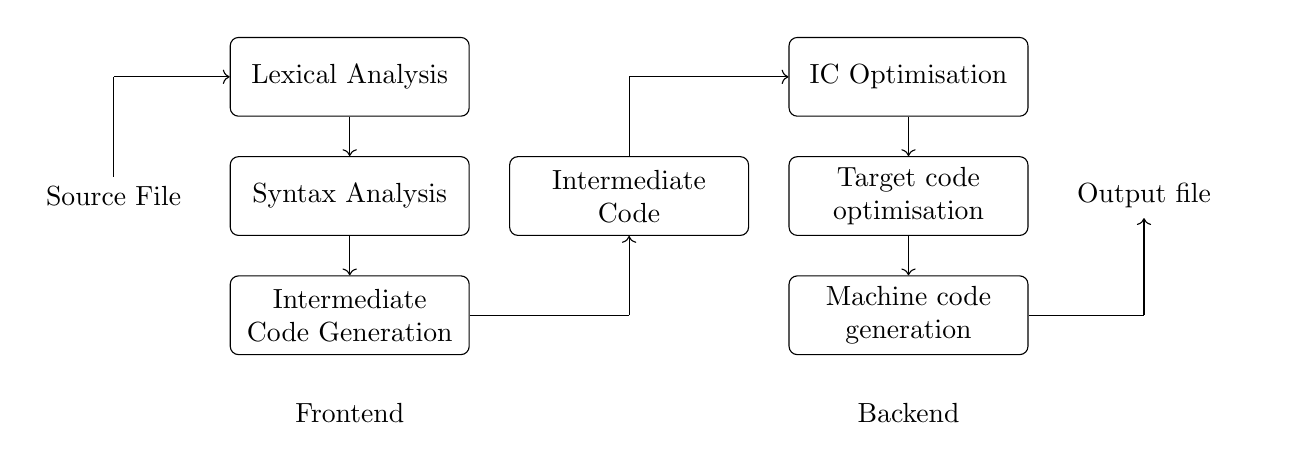
\begin{tikzpicture}
    [
        node distance=4mm,
        block/.style = {
                draw,
                rectangle,
                minimum height=10mm,
                text width=28mm,
                rounded corners=0.3em,
                align=center
            },
    ]

    \matrix[row sep=5mm,column sep=5mm] {
        \coordinate (ul) {};                                     &
        \node [block] (lexer) {Lexical Analysis};                &
        \coordinate (um) {};                                     &
        \node [block] (iopt) {IC Optimisation};                  &
        \coordinate (ur) {};                                     & \\
        \node (file) {Source File};                              &
        \node [block] (parser) {Syntax Analysis};                &
        \node [block] (ir) {Intermediate Code};                  &
        \node [block] (tcodegen) {Target code optimisation};     &
        \node (output) {Output file};                            & \\
                                                                 &
        \node [block] (icodegen) {Intermediate Code Generation}; &
        \coordinate (bm) {};                                     &
        \node [block] (machinecode) {Machine code generation};   &
        \coordinate (br) {};                                     & \\
                                                                 &
        \node (frontend) {Frontend};                             &
                                                                 &
        \node (backend) {Backend};                               &
                                                                 & \\
    };

    \graph[use existing nodes] {
        file -- ul -> lexer -> parser -> icodegen -- bm -> ir -- um -> iopt -> tcodegen -> machinecode -- br -> output;
    };


\end{tikzpicture}
\end{document}
